\subsection{\emph{Docker}}
Dieser Abschnitt behandelt die Verwendung von \emph{Docker}, für das hosten der Services und Datenbanken für die Services. Dank dem \emph{Raspberry PI Image}, bereitgestellt von \emph{Hypriots}, sind bereits \emph{Docker} und \emph{Docker-Compose} \emph{(Orchestration)} vorinstalliert und müssen nicht separat geladen und für die Zielarchitektur gebaut werden.
\newline
\newline
Da der Umgang mit \emph{Docker} und einer umfangreicheren Infrastruktur mit viel Shell-Skripten verbunden ist, wird das Python basierte Tool \emph{Docker-Compose} verwendet, das es erlaubt eine Infrastruktur, die aus einer Menge von untereinander abhängigen Services besteht, deklarativ über eine \emph{YAML}-Konfigurationsdatei zu konfigurieren und zu \emph{orchestrieren}. 
\newline
\newline
Die Definition der \emph{Images} in Form von \emph{Dockerfiles} sowie der Aufbau der \emph{Docker-Compose} Infrastruktur sind im Verzeichnis \emph{$/host/docker/$} enthalten, wobei die einzelnen \emph{Dockerfiles} der Services in Unterverzeichnissen organisiert wurden, die alle Abhängigkeiten, welche in die Images mitaufgenommen werden müssen, enthalten. Die \emph{PostgreSQL} Images stehen am \emph{Docker Hub}\footnote{https://hub.docker.com/r/tobi312/rpi-postgresql/} zur Verfügung. Es wurde ein eigenes Basisimage definiert, das die benötigten Abhängigkeiten für die Interaktion mit der Hardware beinhaltet. Es werden in diesem Basisimage alle benötigten C-Bibliotheken wie \emph{WiringPI}\footnote{https://git.drogon.net/?p=wiringPi;a=summary} und die Bibliotheken für das Interagieren mit der \emph{Raspberry Pi GPU}\footnote{https://github.com/raspberrypi/userland} während des Bauens des Images geladen und für die Zielplattform kompiliert. Das eigenen Basisimage wurde eingeführt, da das Bauen der Abhängigkeiten aufwendig ist und viel Zeit in Anspruch nimmt und sich das Basisimage nur selten ändert.
\begin{center}
	\begin{figure}[h]
		\centering
		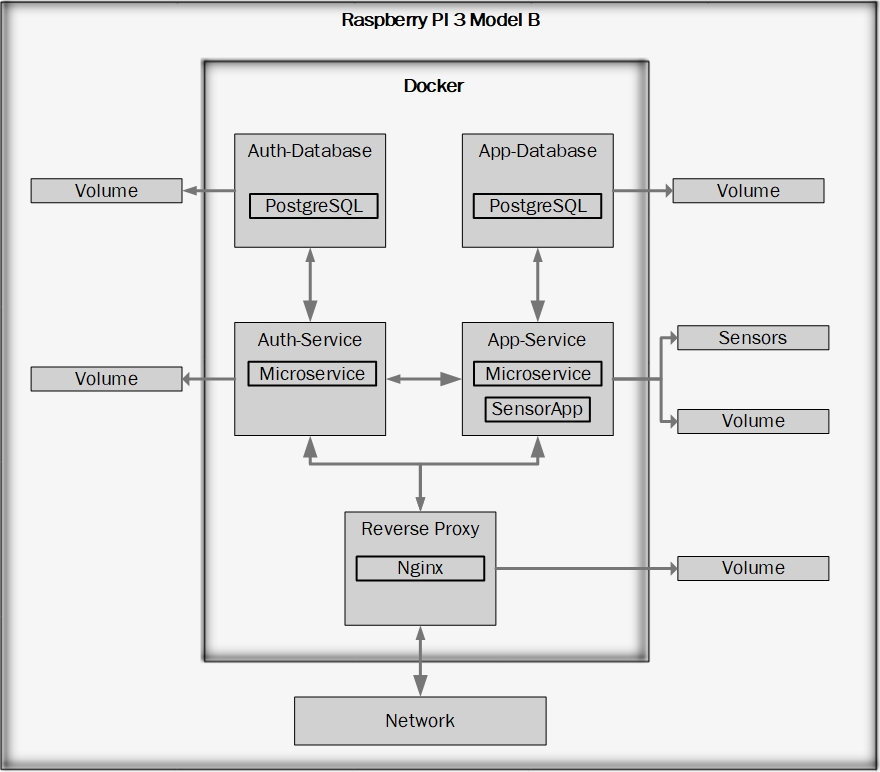
\includegraphics[scale=0.5]{\imageDir/pi-docker-infrastructure.jpg}
		\caption{\emph{Raspberry PI Docker} Infrastruktur}
		\label{fig:rapsi-docker-infrastructure}
	\end{figure}
\end{center}
Die Abbildung \ref{fig:rapsi-docker-infrastructure} zeigt die implementierte \emph{Docker} Infrastruktur, wie sie am \emph{Raspberry PI} gehostet wird. Da die Daten der \emph{Docker-Container} persistent gehalten werden müssen, werden die Daten in den \emph{Containern} in Verzeichnissen gehalten, die auf den \emph{Host} über ein \emph{Volume Mapping} gebunden sind. Der \emph{Docker Container App-Service} benötigt privilegierte Rechte, damit die Sensorapplikation mit der angeschlossenen \emph{Hardware} des \emph{Raspberry PI} kommunizieren kann. 
\newline
\newline
Der Quelltext \ref{src:test-docker-compose} zeigt den Inhalt der \emph{docker-compose.yml}, welche die \emph{Docker} Infrastruktur für \emph{RPISec} am \emph{Raspberry PI} definiert. Die in der Datei vorkommenden Textfragmente im Format \emph{\$\{...\}} stellen Variablen dar, die \emph{Docker-Compose} entweder aus einer Datei mit dem Namen \emph{.env}, die auf derselben Ebene wie die \emph{docker-compose.yml} platziert werden muss, oder aus den Umgebungsvariablen des Benutzers, mit dem die Infrastruktur erstellt wird, auflöst. Sollten Variablen nicht auflösbar sein, so wird eine entsprechende Meldung auf die Konsole ausgegeben.
\begin{code}
	\caption{docker-compose.yml für RPISec am \emph{Raspberry PI}}
	\yamlFile{\dockerRPIDir/docker-compose.yml}
	\label{src:test-docker-compose}
\end{code}
\ \newline
Das Bauen der Infrastruktur und Starten der Services dauert am \emph{Raspberry PI} relativ lange, da nur wenig Speicher zur Verfügung steht, es sich um eine ARM-Architektur handelt und das Speichermedium eine \emph{MicroSD} Karte ist. Ebenso ist die Performance der Services nicht herausragend, jedoch kann die Applikation auf dem \emph{Raspberry PI} problemlos ausgeführt werden.  